\section{Measuring the Cosmological Parameters}

\begin{frame}{Measuring the Cosmological Parameters}{Taylor Expansion of expansion
coefficient}

If we taylor expand a(t) and consider only 2 degree terms

$$ a(t) = a(t_0) + \dot a (t-t_0) + \frac{1}{2} \ddot a (t-t_0)^2 $$

We can define some constants like $H_0 = \frac{\dot a}{a}$, $q_0 = -\frac{\ddot
a}{aH_0^2} = \frac{1}{2} \sum_i \Omega_i (1 + 3w_i)$ (from the acceleration eq).

$$ a(t) = 1 + H_0 (t-t_0) + \frac{1}{2} q_0 H_0^2 (t-t_0)^2 $$

similarly inverse of this can be estimated as:

$$ a(t)^{-1} = 1 - H_0 (t - t_0) + (1 + q_0 /2 ) H_0^2 (t-t_0)^2 $$

This second value is good because we can now calculate the proper distance


\end{frame}

\begin{frame}
	Proper distance in terms of the lookback time $(t_0 - t_e)$ is:
	$$ d_p(t_0) = c \int_{t_e}^{t_o} \frac{dt}{a(t)} = c \int_{t_e}^{t_o}
	(1 - H_0 (t - t_0) + (1 + q_0 /2 ) H_0^2 (t-t_0)^2 ).dt $$
	The $t=t_0$ term cancels out, and only taking upto 2nd degree terms we
	get.
	$$ d_p(t_0) \approx c(t_o - t_e) + cH_0 / 2 (t_0 - t_e)^2 $$

	But the lookback time, is not a good metric that can be easily measured.
	Thus we need to find a way to relate lookback time to redshift.
\end{frame}


\begin{frame}{Measuring the Cosmological Parameters}{Proper Distance}

	If we put $t=t_e$ in the equation.
$$ a(t_e)^{-1} = 1 - H_0 (t_e - t_0) + (1 + q_0 /2 ) H_0^2 (t_e-t_0)^2 $$

And then use the equation $\frac{a(t_0)}{a(t_e)} = 1 + z$, we get
$$ z =  H_0 (t_0 - t_e) + (1 + q_0 /2 ) H_0^2 (t_0-t_e)^2 $$

By inverting the variables we get:
$$ (t_0 - t_e) = H_o^{-1} \left[ z - \frac{1 + q_0}{2}z^2 \right] $$

	Thus the final estimated proper in terms of red-shift distance after
	removing higher degree terms is given by:
	$$ d_p(t_0) = \frac{c}{H_0} z \left[ 1 - \frac{1+q_o}{2} z \right] $$
\end{frame}

\begin{frame}{Measuring the Cosmological Parameters}

	Since we cannot just measure the propper distance from the earth, it
	would be useful to relate it to some known quantities like:

	\begin{itemize}
		\item Standard Candle (Luminosity distance)
			$$ d_L =  \sqrt{\frac{L}{4\pi f}} = d_p(1+z) $$
			Thus proper distance needs to be corrected by a factor
			(1+z)
	$$ d_L(t_o) = \frac{c}{H_0} z \left[ 1 - \frac{1-q_o}{2} z \right] $$
		\item Standard Yardstick ( Angular diameter distance )

			$$ d_A =  \frac{l}{\partial \theta} = d_p/(1+z) $$
			Thus proper distance needs to be corrected by a factor
			1/(1+z)
	$$ d_A(t_o) = \frac{c}{H_0} z \left[ 1 - \frac{3+q_o}{2} z \right] $$

	\end{itemize}
\end{frame}

\begin{frame}{Measureing the Cosmological Parameters}{How to actually calculate}
	Astronomers usually choose the  luminosity distance instead of the
	angular diameter because of lack of proper yardsticks. We have
	extensively used stars called Cepheids whose luminosity keeps
	flucutating in periods, and also IA supernova stars to calculate higher distances
	since they act as good Standard candles with high luminosity.

\begin{columns}[c]
    \column{.5\textwidth}
        \begin{center}
            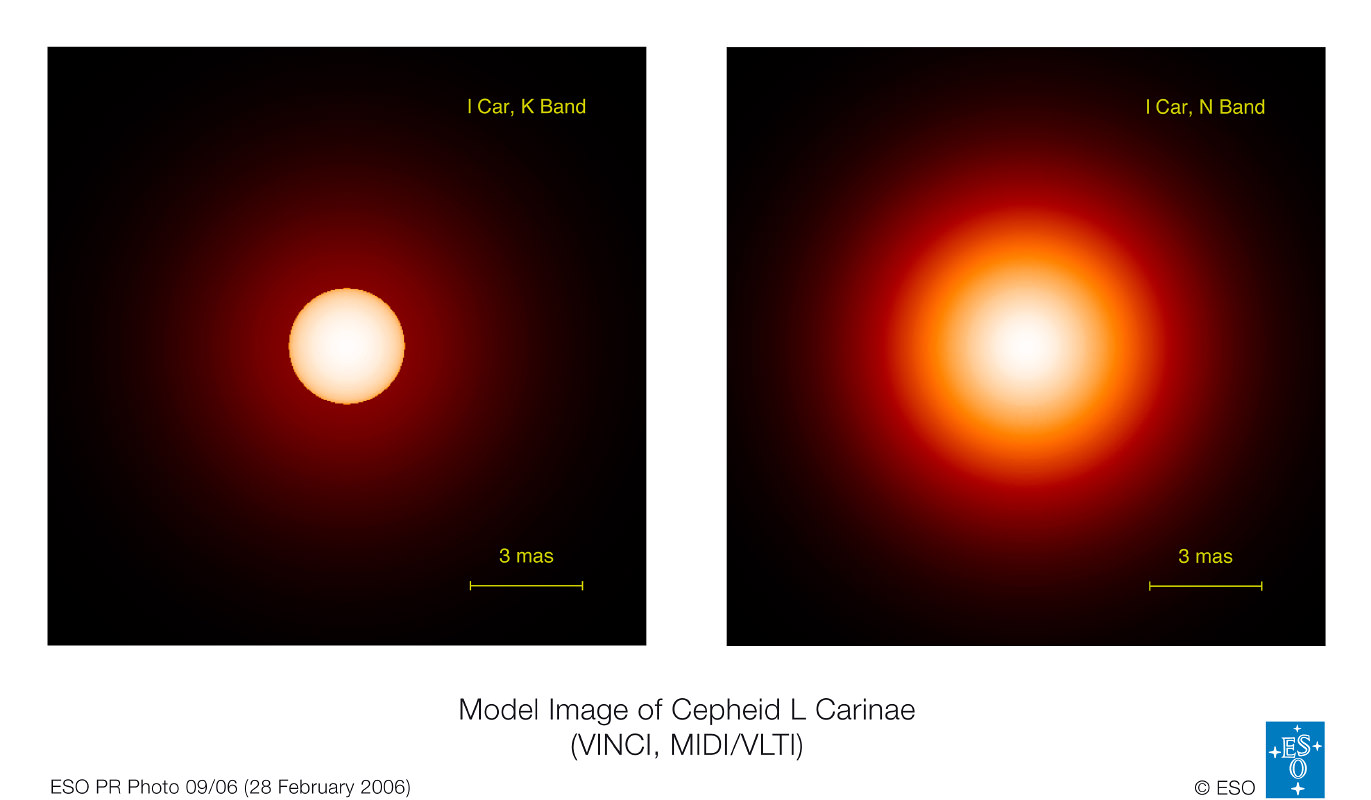
\includegraphics[width=\textwidth]{cepheid.png}
        \end{center}
    \column{.5\textwidth}
        \begin{center}
             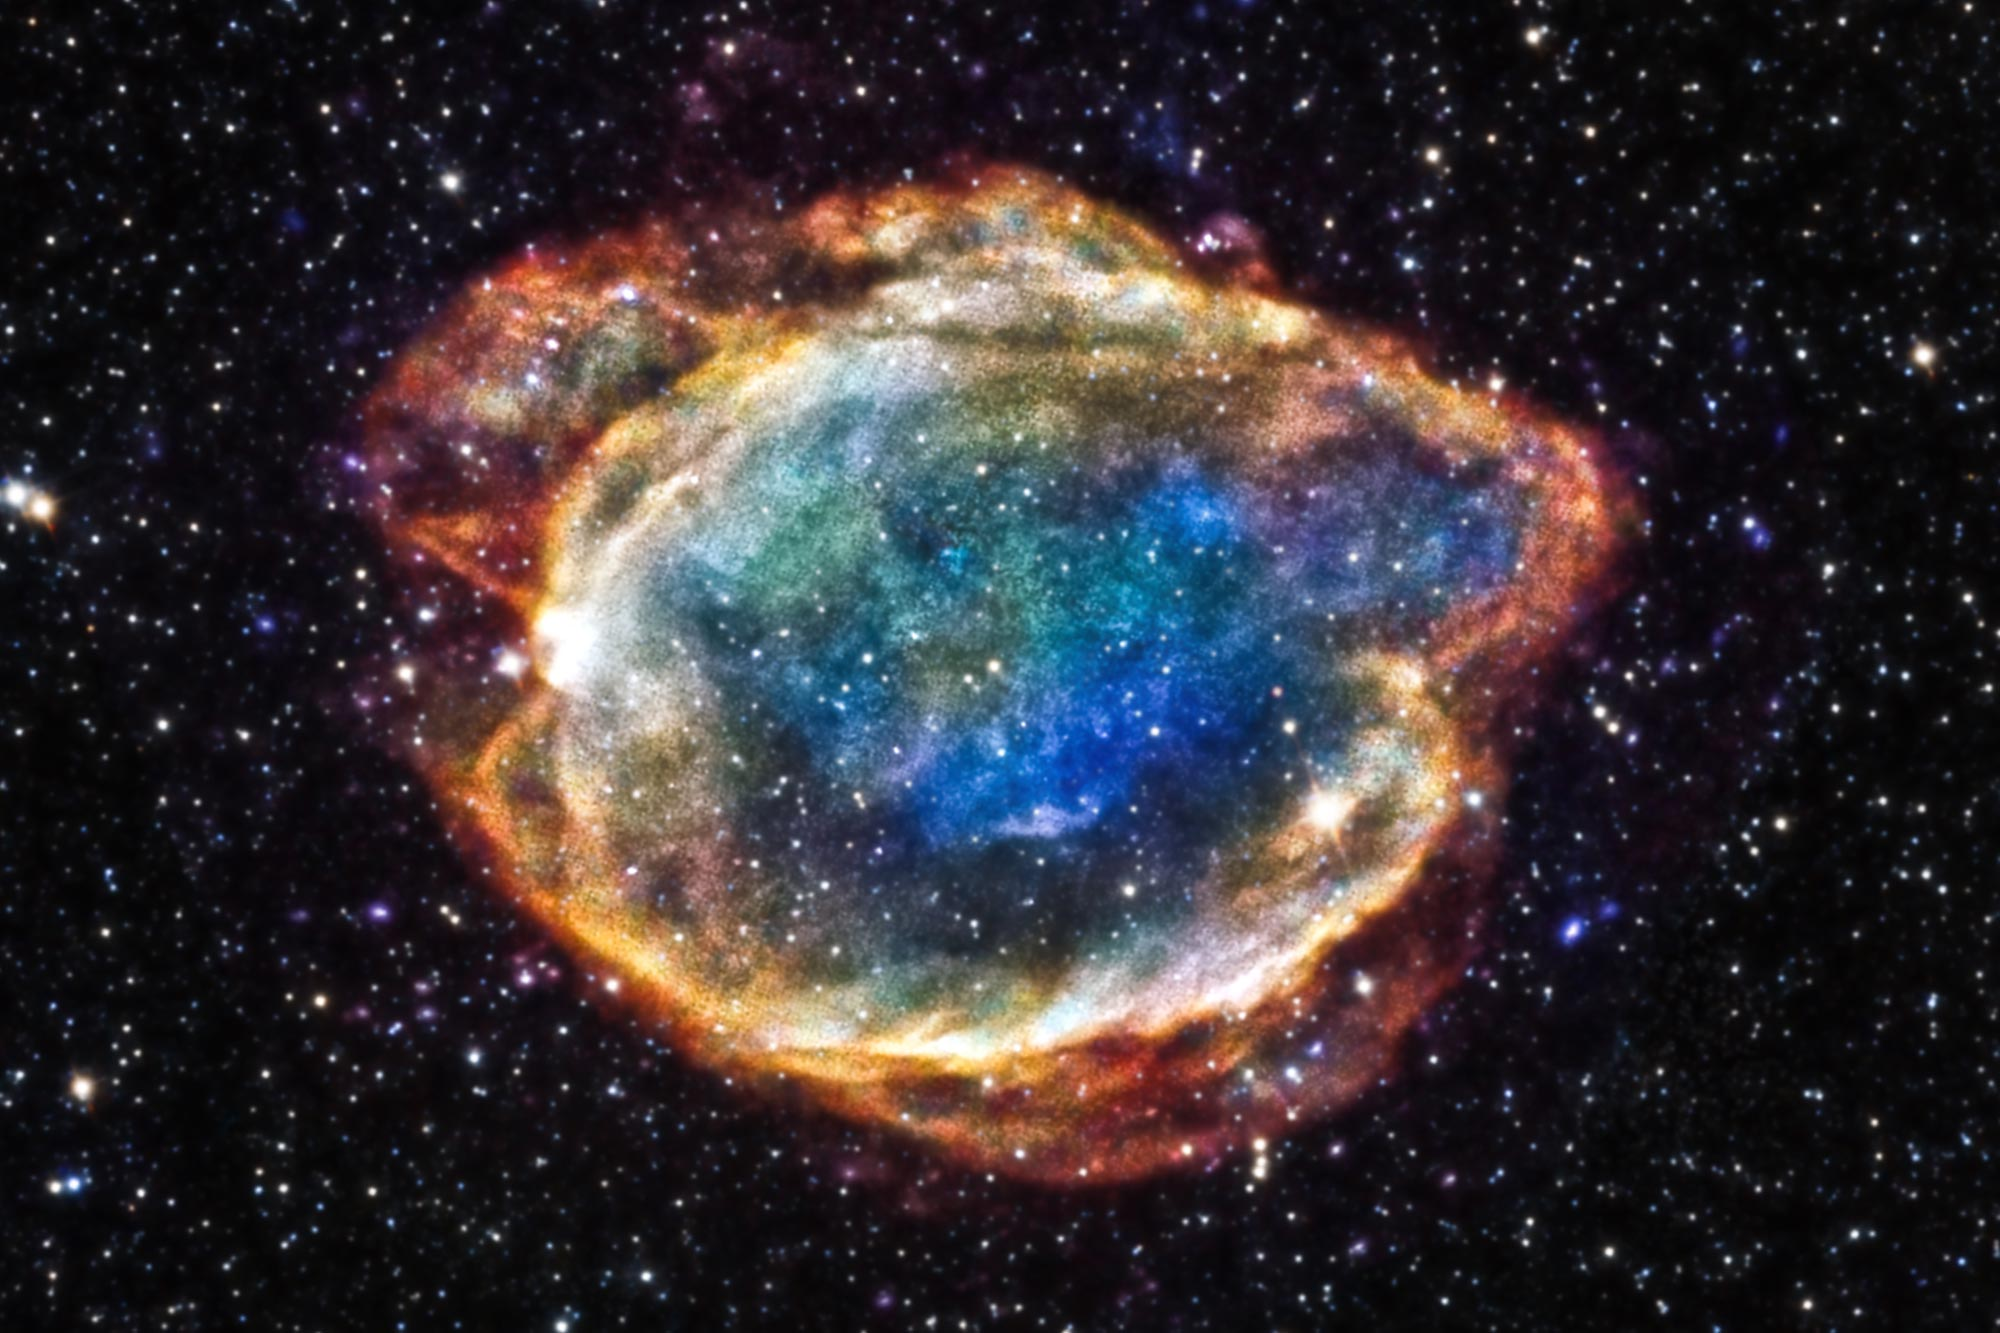
\includegraphics[width=\textwidth]{supernova.png}
        \end{center}
\end{columns}

\end{frame}

\begin{frame}
	It was observed that the luminosity observed by a human eye is in
	logarithmic scale, which also has a historical significance of Greeks
	dividing stars into different apparent brightness scales.

	\begin{enumerate}
		\item Thus the
			\textbf{apparent magnitude} of a light source is defined in terms of the source's
	bolometric flux
	$$ m = -2.5 \log_{10}(f/f_x) $$

\item Similarly we define \textbf{absolute magnitude} of a light source is
	defined wrt. to the apparent magnitude when its distance $d_L = 10 pc$
	$$ M = -2.5 \log_{10}(L/L_x) $$

	Thus we can find luminosity distance using these metrics as:
	$$ m - M = 5 log_{10} \left( \frac{d_L}{1 Mpc} \right) + 25$$

        \end{enumerate}
\end{frame}
